\section{Introduction}

TLS supports user advertised lifetimes of ephemeral secrets. For example, a client can specify that their session key should be deleted after 1 hour to maintain a higher degree of forward secrecy.

The authors made TLS 1.2 handshakes over a nine week period with the Alexa Top Million sites and studied the reuse of private ephemeral values in TLS session resumption, TLS session tickets, and Diffie Helmann key exchange. In addition, the researchers observed more general trends such as the churn of the top million sites and protocol usage statistics. In this report, I present a reproduction of these results two years after the papers publication. Due to time constraints, the data collected spans a comparatively smaller two week period compared to the ninety day period of the original paper.

The key results of this paper which I reproduce correspond to Figures 2-4 in the paper.  Figures 1-2 demonstrate how compliants sites are with these advertised ephemeral lifetimes. Figures 3-4 show how long (in days) that session ticket encryption keys are reused by sites. Reuse of encryption keys expose users to additional risk because it requires that the server save a copy of these keys for their lifetime. Thus, if a malicious party gains server-side access to a site which reuses keys for one week, client communications during the past week can be retroactively decrypted. Additionally, I present a summary of what TLS features are supported by popular domains (e.g. "of the Majestic Million websites that support HTTPS, 83\% support session ID resumption and 76\% support session tickets.") This data for this analyisis was collected over a one week day period from May 26 to June 2.

\section{Data Source}
A verbose json transcript of each TLS handshake used in the analysis is included in this reproduction's Google Cloud Storage bucket (identifier cs244-jared13-tls-crypto). In total, X TLS handshakes were collected across X distinct domains over a period of 14 days. Only X domains remained in the Top Million for the entire X days. Of these, X ever completed a TLS handshake with a browser-trusted certificate. The distribution of the {:,} failed connections is as follows: TABLE


\subsection{Churn}


\begin{figure}[tp]
\centering
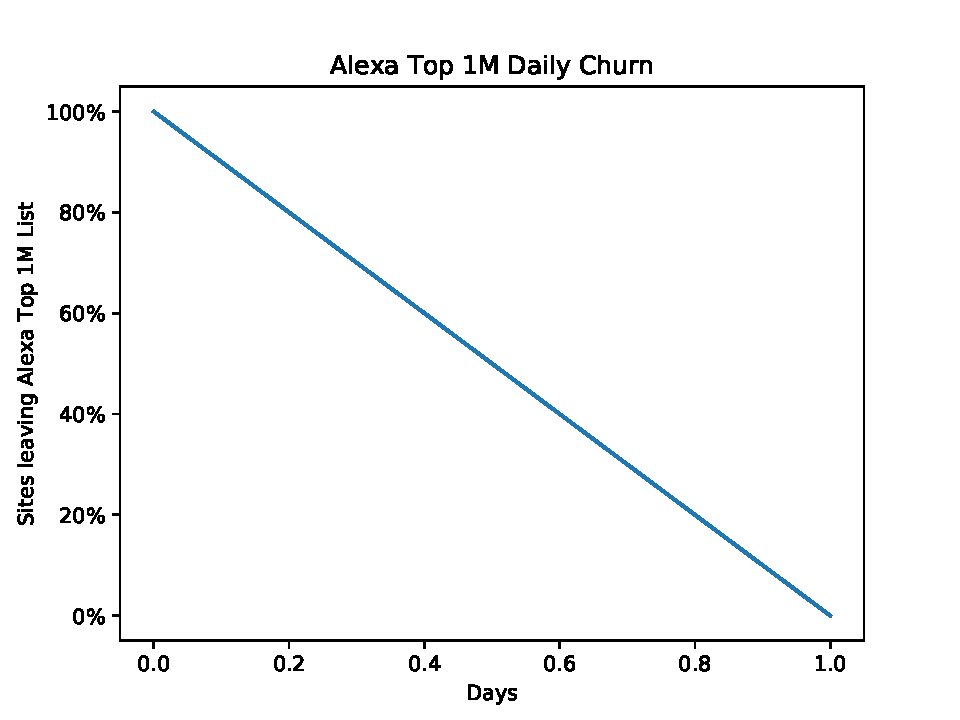
\includegraphics[width=\linewidth]{figures/churn.png}
\caption{\blindtext}
\end{figure}


\section{Reproductions}

\subsection{Figure 2}

Figure 2
\begin{figure}[tp]
\centering
\includegraphics[width=\linewidth]{figures/stek_minutely_cdf.png}
\caption{\blindtext}
\end{figure}

\subsection{Figures 3-4}
Figure 3
\begin{figure}[tp]
\centering
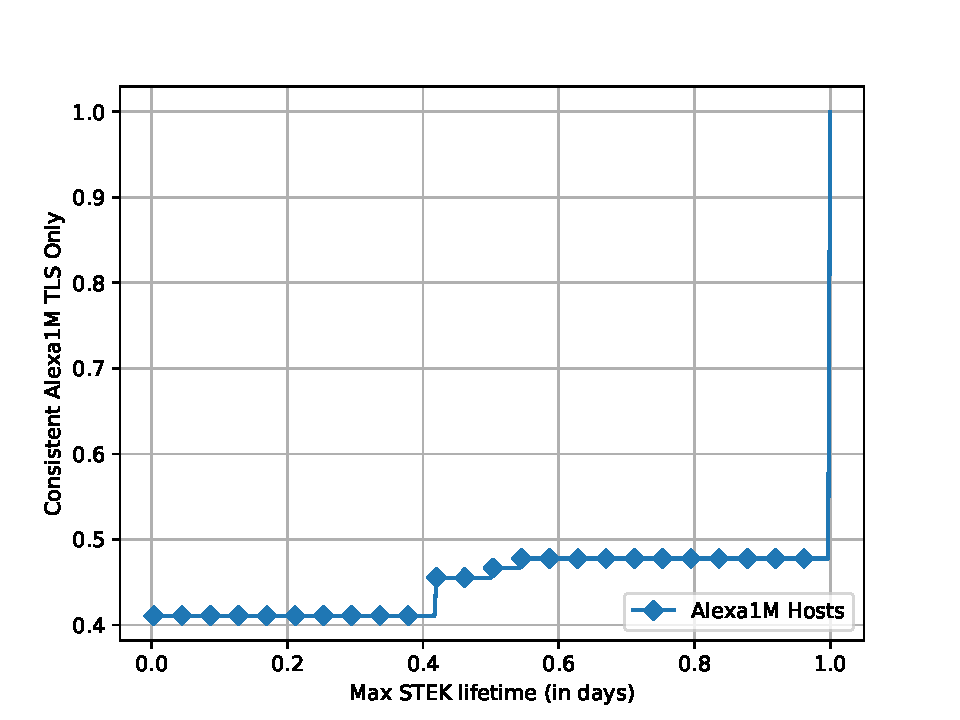
\includegraphics[width=\linewidth]{figures/max_stek_cdf.png}
\caption{\blindtext}
\end{figure}

Figure 4
\begin{figure}[tp]
\centering
\includegraphics[width=\linewidth]{figures/stek_stacked.png}
\caption{\blindtext}
\end{figure}

\section{Evaluation}

\section{Conclusion}